%%%%%%%%%%%%%%%%%%%%%%%%%%%%%%%%%%%%%%%%%%%%%%%%%%%%%%%%%%%%%%%%%%
%%%%%%%%			BACKGROUND
%%%%%%%%%%%%%%%%%%%%%%%%%%%%%%%%%%%%%%%%%%%%%%%%%%%%%%%%%%%%%%%%%%

\section{Background \& Literature Review}

%%\subsection{Introductory Statement}
%%\paragraph{} 
%%Due to my personal experience working as a trainee electrical engineer for an electrical contractor I have a stronger understanding of power systems in the construction industry than most students at my level. This project will be focusing on a designs and simulations to produce deliverables.  

%%%%%%%%%%%%%%%%%%%%%%%%%%%%%%%%%%%%%%%%%%%%%%%%%%%%%%%%%%%%%%%%%%
%%%%%%%%			LITERATURE REVIEW
%%%%%%%%%%%%%%%%%%%%%%%%%%%%%%%%%%%%%%%%%%%%%%%%%%%%%%%%%%%%%%%%%%

\subsection{Literature Review}

\subsubsection{Direct Current vs Alternating Current}

\paragraph{}
A very broad and contextual understanding must be made about the differences be-
tween direct current and alternating current distribution systems. Compared with tradi-
tional AC designs, DC has the potential for effective power supply, smaller feeder
loss, increased efficiency, more consistent power and direct access to renewable
energy solutions \cite{Liu2014}. Alternating current is run to outlets at 240 V AC, 50 \si{Hz} and then devices are used to alter that source into whatever the device requires. Many house-
hold electronics such as computers, chargers, lighting and televisions operate internally
at DC voltages meaning they each require either internal conversion circuitry or use a
transformer between the powerpoint and device \cite{Paajanen2009}.

\paragraph{}
AC was originally depicted as the better choice for power distributions due to there
being no method at the time for controlling DC electricity at the load causing large
losses from the generator to device \cite{Starke2008b}. To remedy this, AC distribution was used
due to efficient transformers being developed to boost the voltage. AC remains the
fundamental power type but DC is growing in popularity with improved converters and
increased frequency of DC energy sources \cite{Starke2008b}. Utilising DC generation systems could
also fulfill the power industry's obligation to increase the sustainability of their systems
and be more environmentally conscious \cite{Starke2008a}. The required converters to change the AC
supply into DC for electronics reduces the efficiency (increasing voltage drop) of the
overall system \cite{Starke2008b}.    

\subsubsection{Low Voltage Direct Current}

\paragraph{}
DC power is currently restricted to special applications such as telecommunications, electric vehciles and high-voltage direct current (HVDC) transmission \cite{Salomonsson2007}. Low-voltage DC power systems at 48 V DC has been used fairly widely with telecommunications systems but is recently facing issues due to the high power requirements of computer system upgrades \cite{Salomonsson2007}. Studies have shown that the 48 V DC system still remains more efficienct than a 270 V DC or 200 V AC but further investigation needs to be done into 230 V DC and 325 V DC through retrofitting existing low voltage AC installations \cite{Salomonsson2007}. Photo-voltatic generators are used frequently for these forms of power distribution systems as it can be powered directly or use simple DC to DC converters for different devices. Utilising a DC distribution system makes it easier to incorporate local power generation. This reduces costs and local power us unaffected by issues with power grid \cite{Starke2008a}. 

\subsubsection{Low Voltage Direct Current in Telecommunications}

\paragraph{}
Using low voltage energy distribution grids for high-speed communications networking which can open up the possibility to utilities for expandsion of widespread local area networks \cite{Waldeck1998}. This could be services such as telephony and internet access without the necessity of additional cabling \cite{Waldeck1998}. Firstly, this voltage level is chosen due to it being marginally under the maximum for low voltage power and still considered a "safe low voltage". Additionally, this voltage level could be backed up by battery systems with four 12 \si{V} batteries in series similar to Figure \ref{fig:48VTelecomms}. Many data centres or communications rooms for corporate buildings will establish arrays of 48 \si{V} battery banks \cite{website:48VTelecomms}. A solution for areas without large enough storage areas for are limited and power demands are low a single 12 \si{v} battery with a 12 \si{V} to 48 \si{V} boost converter can be used \cite{website:48VTelecomms}. This setup is shown in Figure \ref{fig:48VTelecomms}. Additionally, due to this nature of power telecomms, standalone systems are becoming a more suitable means of supply \cite{Ribeiro2009}. Photovoltaic arrays, due to their DC source nature, could be used with a DC to DC boost converter and regulator to power these systems.   

\begin{figure}[H]
\hfill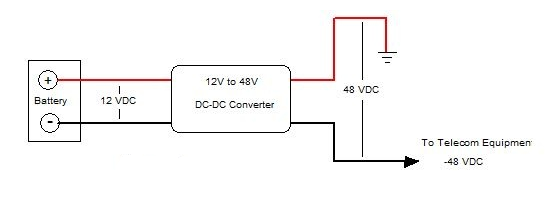
\includegraphics[width = 100mm]{images/12V_Telecomms}\hspace*{\fill}
\caption{Single Battery Communications Room \cite{website:48VTelecomms}}
\label{fig:48VTelecomms}
\end{figure}   

\subsubsection{Existing Power Distribution Systems}

\paragraph{}
Power systems consist of four major sections; generation, transmission, distribution and loads shown in Figure \ref{fig:ExistingPower}. AC electricity is generated in power plants and sent through high voltage transmission lines to substations and distributed to switchboards for use in residential, commercial and industrial areas \cite{Amin2011}. In order to transport electricity over large distances (excess of 2km) without severe losses, very high voltage and low current is used \cite{Amin2011}. This is voltage is lowered and current increased by a transformer at the substation and again at the residence. For electricity to reach the home and be utilised for devices there must be safety mechanisms installed to ensure damage is not done to the user or devices. The protective devices requiring consideration throughout this project will be fuses, circuit breakers and switchboards \cite{UnitedStatesDepartmentoftheInterior2000}. These devices are placed through the circuit to protect the more expensive equipment closer to the transformer and grid.  

\begin{figure}[H]
\hfill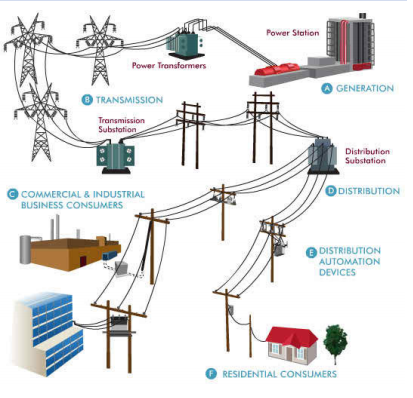
\includegraphics[width = 100mm]{images/Power_Distro}\hspace*{\fill}
\caption{Existing Power Distribution Methods \cite{Active2015}}
\label{fig:ExistingPower}
\end{figure}

\subsubsection{Commercial and Industrial Power Systems}

\paragraph{}
There are relatively large differences between home and commercial power systems. A home application is fairly simple wih a transformer feeding electricity into one distribution board or switchboard (DB) that provides safety mechanisms along with circuit breakers for the home circuits. In a commercial setting, the loads are far higher and require a stable connection \cite{Baran2003}. For an apartment complex, shopping centre or business building, the supplies are generally separated into buses in order to identify separate requirements or areas. The requirements could be essential items (including emergency lifts, safety equipment or machines that cannot be stopped) or non-essentials (tenancies or general equipment). Additionally it can be used to separate the entire building's load over towers or zones to minimise faults. Figure \ref{fig:SLD} represents a single line diagram showing the two separate buses for a design. 

\begin{figure}[H]
\hfill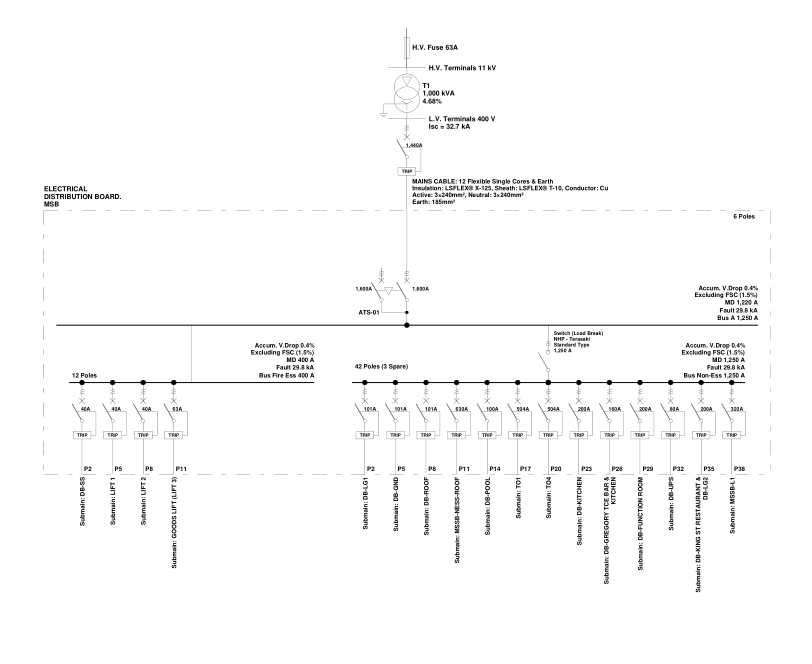
\includegraphics[width = 160mm, height = 110mm]{images/PCad_SLD}\hspace*{\fill}
\caption{{Hotel Single Line Diagram}}
\label{fig:SLD}
\end{figure}       

\subsubsection{Alternative Electricity Generation Solutions}

\paragraph{}
In order to increase efficiency of power systems through utilising a low voltage DC sub-system, alternatives to drawing standard AC electricity from the grid must be considered. In Australia, a strong option for the generation alternative is photo-voltaic systems (known commonly as solar panels). These systems will convert the sun’s rays into electricity and power devices via a regulator, a DC to DC converter \cite{Pillay2004}. This converter is designed to allow the panels to power varying DC loads. If the panels are being used for AC loads, an inverter will also be required. Additionally, if the system is stand-alone a battery will also be required. For the purpose of this project, a vital aspect of DC distribution is the removal of the inverter allowing for the removal of losses caused by these circuits.   

\subsubsection{Photo-Voltaic Arrays and DC Arcing}

\paragraph{}
With the popularity of PV systems increasing, the risk of DC arc faults are being analysed further \cite{Spooner2008}. PV arrays and power systems are being designed with converters boosting voltages to 800 V DC and 1000 V DC. This is being done for efficiency and cost reduction purposes however it leads to large amounts of stress on insulation systems and arc faults developing \cite{Spooner2008}. This causes more safety concerns than traditional AC systems. There are three major causes of arc fault risk; high DC voltage, high DC current and large distribution of DC wiring \cite{website:DC-Arching}.

\paragraph{}
Photovoltaic generators are non-linear sources that vary with intensity of sunlight and behave mainly as a DC current source \cite{Ribeiro2009}. \textbf{Explain DC Arcing}        

\subsubsection{Electrical Safety Mechanisms}

\paragraph{}
For electricity to each the home and be utilised for devices there must be safety
mechanisms installed to ensure damage is not done to the user or devices. The protective
devices requiring consideration throughout this project will be fuses, circuit breakers
and switchboards \cite{UnitedStatesDepartmentoftheInterior2000}. These devices are placed through the circuit to protect the more expensive equipment closer to the transformer and grid. A fuse is a simple device that acts as a sacrificial lamb for the protection of the more expensive devices. An internal wire will melt when too much current flows through therefore interrupting the connection
\cite{UnitedStatesDepartmentoftheInterior2000}. A circuit breaker is a smarter and re-useable version of a fuse that is triggered by overcurrent, overloads or shirt circuits to fulfil the same purpose \cite{UnitedStatesDepartmentoftheInterior2000}. The switchboard is
a device that connects a home or building to the electrical grid and allows for individual
circuits to be run for different purposes throughout the complex \cite{UnitedStatesDepartmentoftheInterior2000}.

\subsubsection{Electrical Safety in Low Voltage DC}

\paragraph{}
Fuses, mechanial and electronic safety switches / circuit breakers and their combinations operate the same in DC as they do in AC; detecting electric faults and switching off to isolate electrical equpment \cite{Meckler2014}. Plugs, sockets and safety equipment with nominal currents of 20 \si{A} are commercially available for pre-existing DC data centres \cite{Meckler2014}. 

\subsubsection{Converters}

\paragraph{}
Converters are electrical devices designed and constructed to convert current between AC and DC \cite{website:ConvVsInverter}. Rectifiers are used to convert the voltage from AC to DC and inverters converter from DC to AC \cite{website:ConvVsInverter}. Although these are the technical terms for the two devices, in general the term "converter" can be used. A specific use for inverters is to convert the DC electrical generated from solar panels to AC for transfer back into mains or to the necessary switchboard. An additional use for these is in Uninterrupted Power Supplies (UPS) where stored DC battery power \cite{website:ConvVsInverter}.

\subsubsection{Buck and Boost Converters}

\paragraph{}
Buck and boost converters are a subset of the converter section above. These are used in DC to DC power systems where the voltage needs to be stepped up or stepped down \cite{textbook:Abu-Rub2014}. For smaller applications, chips such as the LM2575 buck converter are available to reduce voltages according to a feedback. Boost converters do the opposite and increase the voltage. These devices are frequently used with Photo-Voltaic systems depending on what loads they are feeding \cite{textbook:Abu-Rub2014}. The panels generate electricity that is fed through a boost converter then into an inverter to change to AC in order to be distributed throughout the load for standard use \cite{textbook:Abu-Rub2014}.     


\subsubsection{Standards}

\paragraph{}
Australian standards will be an integral part of this project. If the rules and regulations are not adhered to, the devised system will not be legally approved for installation. There are four standards that will be relevant to this report; AS3000, AS3008, AS1680 and AS3015. The AS/NZS 3000 covers the standards related to electrical installations or wiring rules within Australia and New Zealand \cite{StandardsAustralia2007}. These standards will be the main reference point. The AS/NZS 3008 which are the regulations specifically related to electrical installations and cable specifications will be vital \cite{StandardsAustralia2010}. An additional set of standards that will be used for initial calculations and estimation of building load requires is AS/NZS 1680 which are the lighting regulations and requirements for interiors and workplaces \cite{StandardsAustralia2006}. These standards outline the lux levels required by rooms depending according to their purpose allowing 3D models to be created. The AS/NZS 3015 specifically dictates the rules with regards to electrical installations of extra low voltage direct current power supplies and services earthing within public telecommunications \cite{StandardsAustralia2004}.     

\subsubsection{Tariffs}

\paragraph{}
Tariffs will be an important consideration with the feasibility of this project due to the
possibilities of cost reduction. User expenses could theoretically be reduced by imple-
menting a system off the grid. Government policies have been put in place in order
to prompt an increase in investment in renewable energy sources \cite{Nelson2011}. Users are able to sell their unused generated electricity back to the grid to reduce their overall electricity
bills or possibly profit if consumption is low enough. In Queensland, according to the
SolarChoice website a feed-in tariff of \$0.06/kWh can be earned \cite{website:SolarChoice}. By not connecting the photo voltaic panels to the grid, this tariff can not be received however there is the possibility that it is more efficient and will produce less energy loss by storing in local
batteries and running simple circuits rather than feeding the grid \cite{AntoniouATzimasARowland2015}. The consideration will be whether the cost reduction in electricity bill will be worth the investment in the equipment and future cost reduction.   

\subsubsection{LED Lighting}

\paragraph{}
Table \ref{LightingTypes} below shows a technical comparison of three common lighting types. Improvements in LED lighting allow less power to be used for the same brightness. It is possible to design and create an energy efficient LVDC grid powered LED lighitng system with additional automation aspects and energy storage \cite{Koh2011}. Typical lighting systems are flurescent bulbs or tubes that are powered directly from standard 230 V AC due to the devices' high efficacy \cite{Koh2011}. When comparing an AC flurescent system and a LVDC LED system, the LVDC gid system requires sigificantly less power conversion which increases the overall effiency \cite{Koh2011}. The table below represents these factors. For applications, this means less physical lights are necessary for equivalent light reducing project costs \cite{website:LED}.  

\begin{table}[!ht]
\centering
\renewcommand{\arraystretch}{2} % Changing spacing
\begin{tabular}{|l|c|c|c|}
\hline
\textbf{Lighting Type (Bulbs)} & \multicolumn{1}{l|}{\textit{Incandescent}} & \multicolumn{1}{l|}{\textit{CFL}} & \multicolumn{1}{l|}{\textit{LED}} \\ \hline
Average Lifespan (hours) & 1,200 & 8,000 & 50,000 \\ \hline
Wattage (at 800 lumens) & 60 & 13-15 & 6-8 \\ \hline
Lumens/Watt & 13.3 & 53.3 & 114.3 \\ \hline
\end{tabular} \quad
\caption{Comparing Efficiencies of Lighting Types (Bulbs) \cite{Koh2011}}
\label{LightingTypes}
\end{table}





\newpage